% Chapter Template

\chapter{X-ray luminosity - age relationship} % Main chapter title

\label{Chapter3} % Change X to a consecutive number; for referencing this chapter elsewhere, use \ref{ChapterX}

%----------------------------------------------------------------------------------------
%	SECTION 1
%----------------------------------------------------------------------------------------

\epigraph{\itshape There are only four rules you need to remember: make the plan, execute the plan, expect the plan to go off the rails, throw away the plan.}{---L. Snart, \itshape The Flash}

\section{Introduction}
The work presented in this chapter was published in the Monthly Notices of the Royal Astronomical Society, Volume 471, p.1012-1025 as the article entitled "An improved age-activity relationship for cool stars older than a gigayear" \citep{Booth_etal_2017} and modified here to fit within the framework and context of this thesis. This chapter discusses the work conducted in \citet{Booth_etal_2017} in greater depth. \textcolor{red}{Insert here if I have discussed anything that wasn't in the paper}. The aim of this study was to investigate the age-activity relationship beyond a gigayear using X-ray luminosity as a magnetic activity indicator and asteroseismology as the source for stellar ages.

\subsection{Chandra and XMM-Newton telescopes}
This study utilises observations from the Chandra and XMM-Newton X-ray telescopes which are space-based telescopes in highly eccentric orbits around Earth. This places the telescopes in an ideal position to perform long, uninterrupted observations necessary in the X-ray regime. It is worth mentioning that X-ray telescopes are unlike traditional optical telescopes in their setup. Since X-ray radiation passes through most material, the mirrors must be positioned almost parallel to the incoming photons. This causes the X-ray photons to reflect off the mirror at a grazing incidence, this process is repeated with a secondary mirror in order to focus the X-ray light to a focal point as shown in Figure \ref{fig:diagram_xray_telescope}.

\begin{figure}
    \centering
    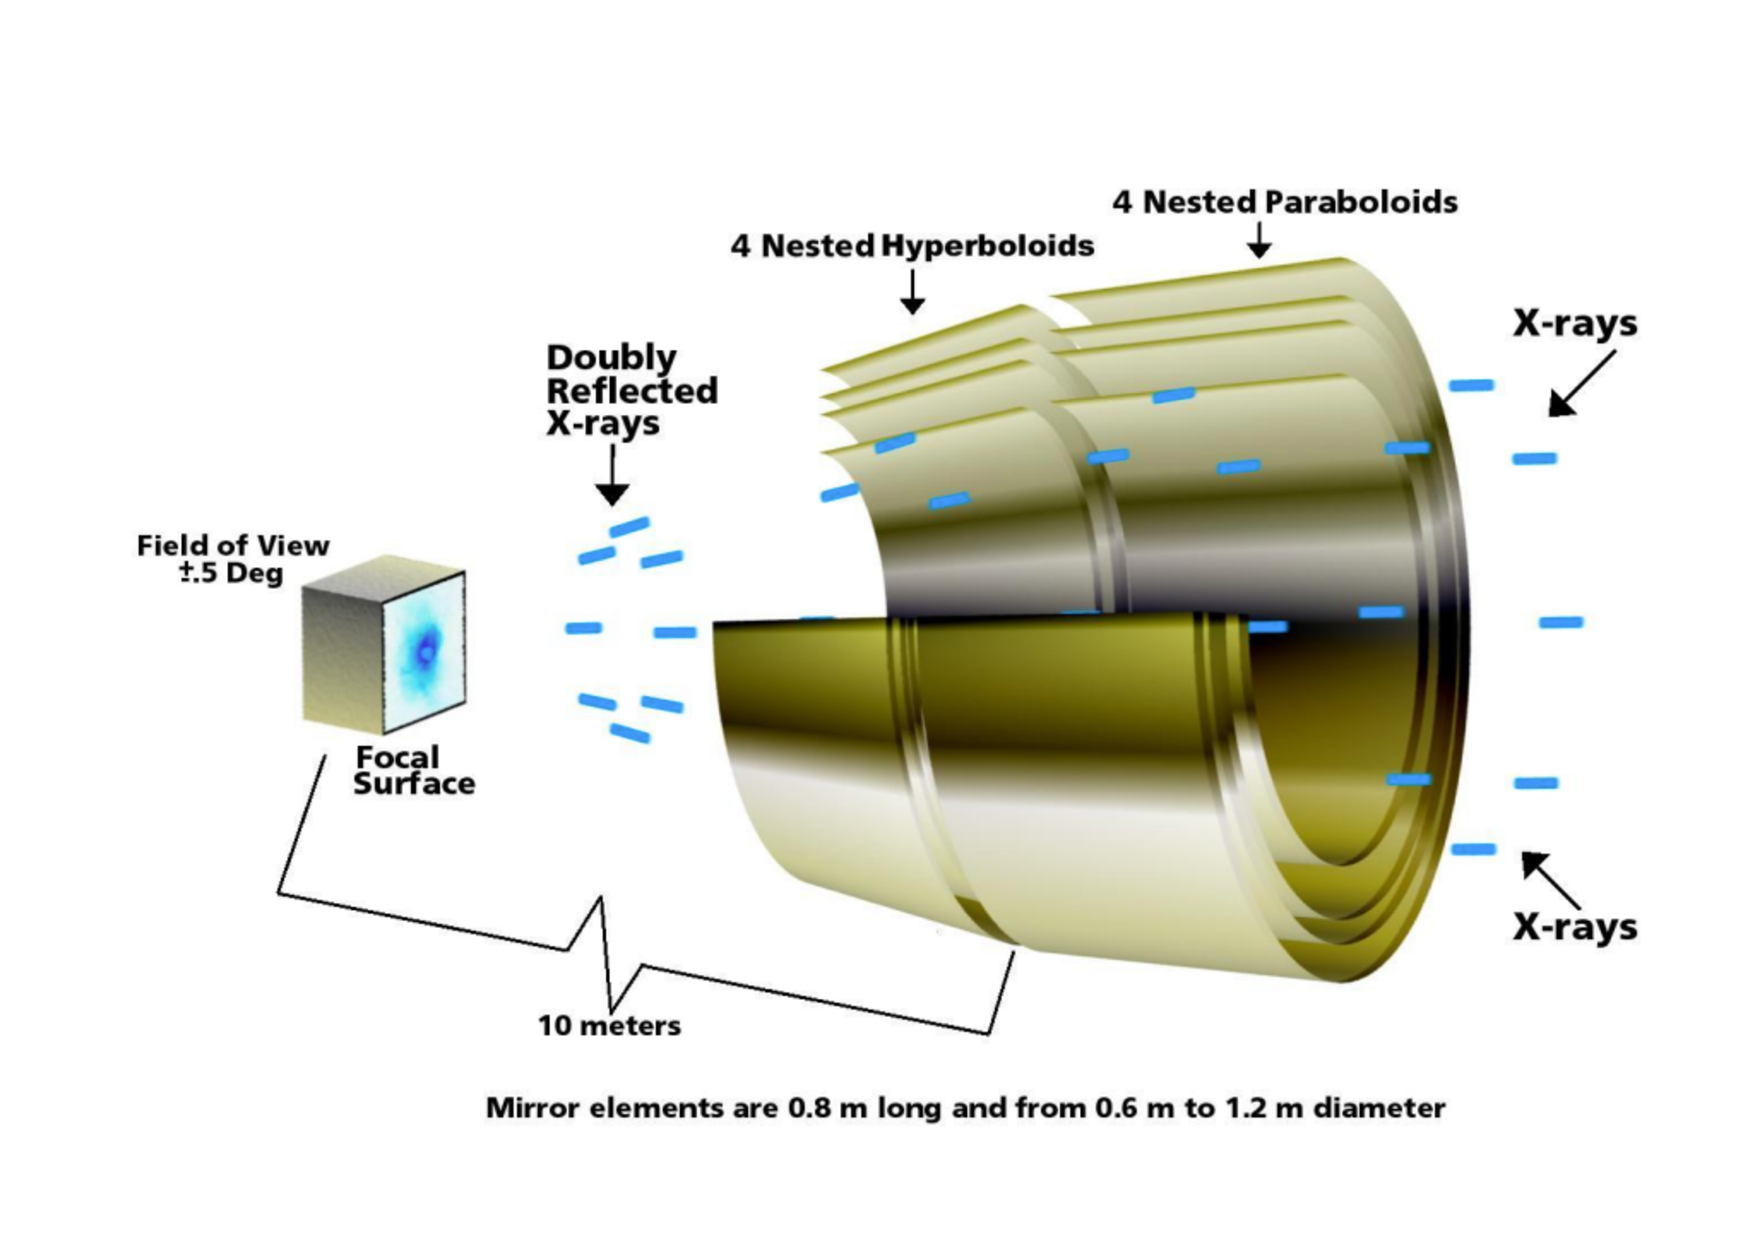
\includegraphics[scale=0.45]{Figures/3-Xray_age/chandra_scheme.pdf}
    \caption{Schematic of Chandra X-ray telescope. Four nested co-axial, confocal, grazing incident mirrors focus the X-ray photons to a common focal point where the detectors are located. Image Credit: NASA/CXC/ D. Berry}
    \label{fig:diagram_xray_telescope}
\end{figure}

The XMM-Newton X-ray telescope \citep{Jansen_etal_2001} contains three x-ray CCD cameras collectively known as EPIC. EPIC is made up of one PN detector and two metal oxide detectors (MOS 1 and MOS 2). The MOS detectors are located behind the telescopes grating and only receives approximately half of the incident flux. Whereas the PN detector has an unobstructed beam and a much higher signal to noise than the MOS detectors, therefore data analysis is preferably performed with PN observations. The EPIC instrument is capable of imaging over the telescope's 30 arcmin field of view in the energy range 0.2 - 15 keV (62 - 0.826 \AA). Note that due to the short wavelengths of X-ray radiation, wavelengths are preferably presented in terms of energy. All EPIC CCD's operate in a photon counting mode which produces an event list including the position of photon, arrival time and the photon energy; this allows for both imaging and spectra of X-ray objects.

The Chandra telescope \citep{Weisskopf_etal_2000} has two focal plane instruments: the advanced CCD imaging spectrometer (ACIS) and the high resolution camera (HRC). The HRC provides only images and no spectral information, therefore in this study observations are restricted to ACIS since it provides spectral information in the energy range 0.2 - 10 keV.

\section{Observations and stellar sample}
\subsection{Sample selection}
Our target stars with well-determined ages were selected from several different sources. The majority stems from asteroseismology where stars were chosen with precisely determined stellar parameters, including ages, from modelling of individual oscillation frequencies as observed by the Kepler satellite \citep{Silva_Aguirre_etal_2015,Silva_Aguirre_etal_2017}. However, for some stars the signal to noise was not high enough to model the individual oscillation frequencies. In these circumstances, the global asteroseismic parameters \citep{Chaplin_etal_2014} are combined with spectroscopic parameters ($T_{eff}$ and [Fe/H]) and ages are obtained through \texttt{BASTA} \citep{Silva_Aguirre_etal_2015}. \texttt{BASTA} uses a Bayesian approach to determine the probability that a set of parameters matches the observed asteroseismic parameters.
%Maybe add more in here

The second source



\subsection{Distances and spectral types}

\subsection{Ages of systems with white dwarfs}






































\newpage